\documentclass{article}

\usepackage[margin=1in]{geometry}
\usepackage[utf8]{inputenc}
\usepackage[english]{babel}
\usepackage{amsthm} %lets us use \begin{proof}
\usepackage{amssymb} %gives us the character \varnothing
\usepackage{xcolor}
\usepackage{float}
\usepackage{braket}
\usepackage{multirow}
\usepackage{array}
\usepackage{mathtools}
\usepackage{diagbox}
\usepackage{gensymb}

\title{Chem231B: Hw 4} % Title of the assignment

\begin{document}

\maketitle

\section*{\textbf{BO Approx}}

a) Making the BO approximation, write the purely electronic Hamiltonian and, by
completing the square, write its energy levels $E_{\text{el,n}}(X)$.

\begin{equation}
  \hat{H}_{\text{el}} = \hat{T}_{\text{el}} + V(X,x)
\end{equation}

Given: $V(X,x) = \frac{1}{2}(X^2+x^2) + \frac{1}{2}(x-X)^2$

Rearrange $V(X,x)$ and completing the square,
\begin{align}
  V(X,x) & = \frac{1}{2}(X^2+x^2) + \frac{1}{2}(x-X)^2 \nonumber \\
  & = \frac{1}{2}X^2+\frac{1}{2}x^2 + \frac{1}{2}(x^2-2xX+X^2) \nonumber \\
  & = X^2 + x^2 - xX + 2xX - 2xX \nonumber\\
  & = (x - X)^2 + xX.
\end{align}

Hence, the purely electronic Hamiltonian is,
\begin{align}
  \hat{H}_{\text{el}} & = \hat{T}_{\text{el}} + V(X,x) \nonumber\\
  & = \frac{p_x^2}{2} + (x - X)^2 + xX,
\end{align}

where $p_x$ is momentum operator for the electron. The Sch\"odinger equation
for the electronic part,
\begin{align}
  \hat{H}_{\text{el}}\phi_{\text{el}}(x) & = E_{\text{el,n}}\phi_{\text{el}}(x) \\
  \Bigg(\frac{p_x^2}{2} + (x - X)^2 + xX\Bigg)\phi_{\text{el}}(x)
  & =E_{\text{el,n}}(X)\phi_{\text{el}}(x). \label{eqn:elec}
\end{align}

This looks like the harmonic oscillator problem but with an additional
coupled $xX$ term and proton position $X$ in the $(x-X)^2$ term.
The harmonic oscillator wavefunctions are solutions to Eqn \eqref{eqn:elec}.
For convenience, we rewrite $(x-X)^2=(1/2)(2)(x-X)^2$ and this shows that
$\omega_{\text{el}}=\sqrt{2}$. Throughout the problem, $\omega_{\text{el}}$ will be used
and substituted later. The energy levels $E_{\text{el,n}}(X)$ are determined for $n=0,1$
and then generalized to $n$ levels. At $n=0$,
\begin{align}
  \phi_{\text{el,0}}(x) & = \Bigg(\frac{\omega_{\text{el}}}{\pi}\Bigg)^{\frac{1}{4}}
  e^{-\omega_{\text{el}}x^2/2} \\
  E_{\text{el,0}} & = \langle \hat{T}_{\text{el}}\rangle + \langle V(X,x) \rangle \nonumber \\
  & = \frac{\omega_{\text{el}}}{4} + \frac{\omega_{\text{el}}}{4}(1+2X^2\omega_{\text{el}}) \nonumber\\
  & = \frac{\omega_{\text{el}}}{2} + \frac{X^2\omega_{\text{el}}^2}{2}.
\end{align}

Repeat for $n=1$,
\begin{align}
  \phi_{\text{el,1}}(x) & = \Bigg(\frac{\omega_{\text{el}}}{\pi}\Bigg)^{\frac{1}{4}}
  \sqrt{2\omega_{\text{el}}}\,e^{-\omega_{\text{el}}x^2/2} \\
  E_{\text{el,1}} & = \frac{3\omega_{\text{el}}}{2} + \frac{X^2\omega_{\text{el}}^2}{2}.
\end{align}

Therefore, $E_{\text{el,n}}(X)=(n+\frac{1}{2})\omega_{\text{el}} + \frac{X^2\omega_{\text{el}}^2}{2}$.
\\

\noindent b) Write the nuclear equation for the proton in the field of the
electronic energy plus any other parts of the potential, to get an expression
for the totla energy of the system, $E_{\nu,n}$, where $\nu$ is the quantum
number for proton vibrations.
\\

Given the full Hamiltonian ($\hat{H}$), the full wavefunction ($\Psi(x,X)$),
and the Schr\"odinger equation,
\begin{align}
  \hat{H}\Psi(x,X) & = E_{\text{tot}}\Psi(x,X) \\
  \Psi(x,X) & = \phi_{\text{el}}(x)\phi_{\text{nuc}}(X) \\
  \hat{H} & = \hat{T}_{\text{nuc}} + \hat{T}_{\text{el}} + V(X,x).
\end{align}

Since the electronic part of the wavefunction is solved in part a), the
nuclear part is leftover,
\begin{equation}
  (\hat{T}_{\text{nuc}} + E_{\text{el,n}}(X))\phi_{\text{el}}(x)\phi_{\text{nuc}}(X)
  = E_{\text{tot}}\phi_{\text{el}}(x)\phi_{\text{nuc}}(X). \label{eqn:nuc}
\end{equation}
Solutions of $\phi_{\text{nuc}}(X)$ for Eqn \eqref{eqn:nuc} is simply the harmonic
oscillator wavefunctions. Similarly, in part a), the computation of $E_{\nu}$ for
quantum number of proton vibrations $\nu=0$ is shown,
\begin{align}
  \phi_{\text{nuc},0}(X) & = \Bigg(\frac{m\omega_{\text{nuc}}}{\pi}\Bigg)^{\frac{1}{4}}
  e^{-m\omega_{\text{nuc}}X^2/2} \\
  E_{\nu=0} & = \frac{\omega_{\text{nuc}}}{4} + \frac{3\omega^2_{\text{el}}}{4m\omega_{\text{nuc}}}.
\end{align}

For $\nu=1$, $E_{\nu=1}$ can be computed
\begin{align}
  \phi_{\text{nuc},1}(X) & = \Bigg(\frac{m\omega_{\text{nuc}}}{\pi}\Bigg)^{\frac{1}{4}}
  \sqrt{2m\omega_{\text{nuc}}}\,e^{-m\omega_{\text{nuc}}X^2/2} \\
  E_{\nu=1} & = \frac{3\omega_{\text{nuc}}}{4} + \frac{3\omega^2_{\text{el}}}{4m\omega_{\text{nuc}}}.
\end{align}

Based on these, the total energy ($E_{\nu,n}$) is,
\begin{equation}
  E_{\nu,n}=\Big(\nu+\frac{1}{2}\Big)\frac{\omega_{\text{nuc}}}{2}
  + \Big(n+\frac{1}{2}\Big)\omega_{\text{el}}
  + \frac{3\omega^2_{\text{el}}}{4m\omega_{\text{nuc}}}.
\end{equation}

\noindent c) Assume $m=25$, plot the lowest 12 levels, labeling them with their
electronic and nuclear quantum numbers.
\\

%Given the $E_{\nu,n}$ for $m=25$,
%\begin{equation}
%  E_{\nu,n} = \Big(\nu+\frac{1}{2}\Big)\frac{\omega_{\text{nuc}}}{2}
%  + \Big(n+\frac{1}{2}\Big)\omega_{\text{el}}
%  + \frac{3\omega^2_{\text{el}}}{100\omega_{\text{nuc}}}.
%\end{equation}

From earlier, $\omega_{\text{el}}=\sqrt{2}$ which means that $k=2$. We
can define $\omega_{\text{nuc}}=\sqrt{k/m}=\sqrt{2/m}$. The energy state $(\nu,n)$
is given by,
\begin{align}
  E_{\nu,n} & = \Big(\nu+\frac{1}{2}\Big)\frac{\sqrt{2}}{2\sqrt{m}}
  + \Big(n+\frac{1}{2}\Big)\sqrt{2}
  + \frac{3\sqrt{2}}{4\sqrt{m}} \nonumber\\
  & = \Big(\nu + 2\Big)\frac{\sqrt{2}}{2\sqrt{m}}
  + \Big(n+\frac{1}{2}\Big)\sqrt{2}
\end{align}

\begin{figure}[H]
  \centering
  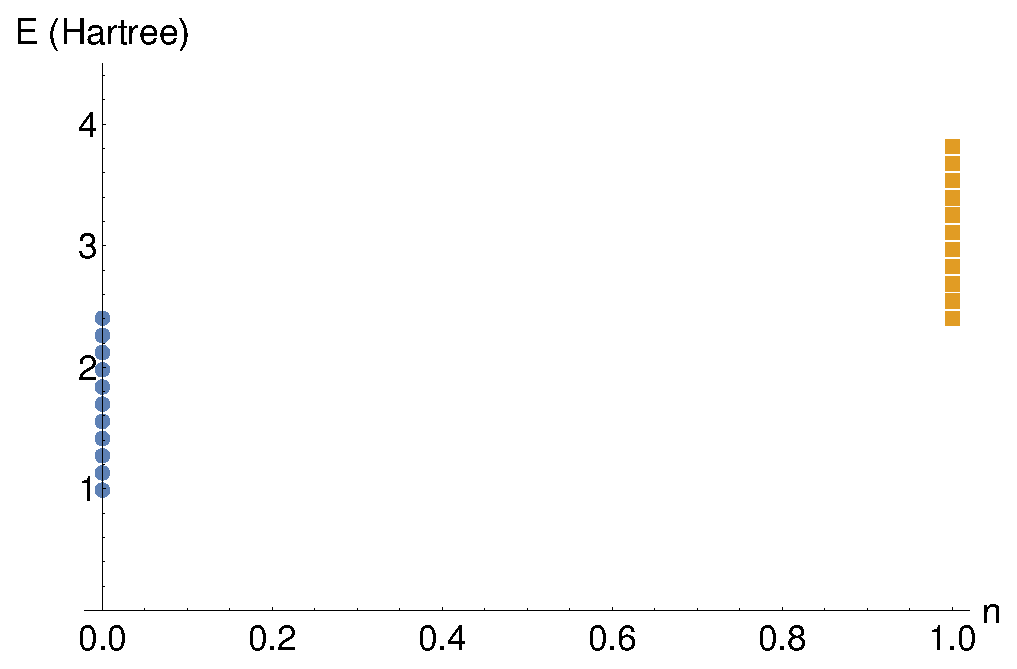
\includegraphics[scale=0.7]{energy_levels.eps}
  \caption{Computed total energy levels ($E_{\nu,n}$) for given nuclear
    and electronic quantum numbers $(\nu,n)$. The first 11 nuclear states
    ($\nu$) are plotted at given $n$.}
  \label{fig:E_levels}
\end{figure}

\begin{table}[H]
  \centering
  \caption{Reported total energy in Hartree ($E_{\nu,n}$) for given nuclear and electronic
    quantum numbers $(\nu,n)$.}
  \begin{tabular}{c|cc}
    \diagbox{$\nu$}{$n$} & 0 & 1 \\
    \hline \\
    0 & 0.990 & 2.404 \\
    1 & 1.131 & 2.546 \\
    2 & 1.273 & 2.687 \\
    3 & 1.414 & 2.828 \\ 
    4 & 1.556 & 2.970 \\ 
    5 & 1.697 & 3.111 \\ 
    6 & 1.838 & 3.253 \\ 
    7 & 1.980 & 3.394 \\ 
    8 & 2.121 & 3.536 \\ 
    9 & 2.263 & 3.677 \\ 
   10 & 2.404 & 3.818
  \end{tabular}
\end{table}

\pagebreak

\section*{General Problems about Diatomics from BRR}

  1. \textit{Ionic bonds:} Use Table 7.3 to deduce the values of B and $\rho$ used in
  Eq (7.43). Are they reasonable? How might you have found them without reverse engineering?
  Is the agreement between calculation and experiment accurate enough by quantum chemistry
  standards? Identify which components of a KS calculation are being approximated by the
  separate terms in Eq (7.44).

  \begin{equation}
    V_{\text{rep}}(R) = Be^{-R/\rho}
    \label{eqn:born_mayer}
  \end{equation}

  Reverse engineering the data requires looking up the $\alpha_i$ polarizability
  of the $i$-th ion from doi:10.1063/1.1679747. Once obtaining those values, the
  ``ionic dissociation energy'' can be computed and an exponential fit can be
  arranged via mathematica. The constants $B$ and $\rho$ are XX and XX, respectively.

  \begin{figure}[H]
    \centering
    \includegraphics[scale=0.5]{fit}
    \caption{Exponential fit for the Born--Mayer potential to determine $B$ and
      $\rho$ from Eqn. \eqref{eqn:born_mayer}}
    \label{fig:fit}
  \end{figure}
  
  \begin{table}[H]
    \centering
    \caption{Ionic Bond Model and absolute difference between experiment and calculated
      in eV.}
    \begin{tabular}{cccc}
      Molecule & Calc. & Obs. & Diff \\
      \hline
      LiF  & 7.9996 & 7.983 & 0.017 \\
      LiCl & 6.513  & 6.648 & 0.135 \\
      NaCl & 5.616  & 5.750 & 0.134 \\
      KF   & 5.993  & 6.036 & 0.043 \\
      KI   & 4.458  & 4.601 & 0.143 \\
      RbCl & 4.835  & 4.917 & 0.082 \\
      CsCl & 4.692  & 4.870 & 0.178
    \end{tabular}
  \end{table}
  
  The error can be up to $\sim 0.2$ eV, or $\sim 3$ kcal/mol. It is fairly good for smaller
  ions within chemical accuracy of $\sim 1$ kcal/mol. However, the model does not do ``well''
  for large ions where errors can reach up to $\sim 3$ kcal/mol based on quantum chemistry
  standards.
  \\
  \\
  \noindent2. \textit{Homonuclear diatomics:} Use Fig 7.14 to identify the error in a configuration
  in Table 7.5. Explain the labeling of the excited states in Table 7.6.
  \\

  According to Fig 7.14, the molecular orbital configuration of N$_2$ is incorrect and it
  should be:

  N$_2$: KK$(2\sigma_g)^2(2\sigma_u)^2(3\sigma_g)^2(1\pi_u)^4$
  \\
  
  Molecular term symbols are defined
  \begin{equation*}
    ^{2S+1}|\Lambda|_{(g/u)}^{(+/-)}
  \end{equation*}
  \noindent where $S$ is the total spin angular momentum, $\Lambda$ is the total orbital
  angular momentum, $g/u$ corrpondes to symmetry of the electronic wavefunction with repect
  to inversion through this center, and $+/-$ applies only to $\Sigma$ states labeling
  symmetry of the wavefunction with respect to the reflection in a plane containing the
  nuclei. 
  \\
  \\
  \noindent3. \textit{Electronegativity:} Read 7.7 and explain the spelling error in FONClBrISCHP.
  \\
  
  Based on the Pauling scale, FONClBrISCHP has the incorrect order from most to least electronegative
  atoms. The correct order is FOClNBrISCHP.
  \\
  
  \noindent4. \textit{Potential energy surfaces:} Read 7.8 and explain the Massey criterion.
  When can curves cross and when do they not? If curves do not cross, can molecules change
  PES?
  \\
  
  The Massey adiabatic criterion is the transition period ($\Delta t$) at which the molecule
  on one potential energy surface (PES) encounters another PES within $\Delta E$ over a range
  $\Delta R$. Yes, the molecule can change PES if the curves do not cross e.g. phosphorescence.
  \\
  \\
  \noindent5. \textit{Hydrides and isoelectronic series:} Read 7.9 and explain what is special
  about diatomic hydrides. Explain how hydrogen bonding upsets trends in boiling point
  data. Do problem 7.20.
  \\
  
  Nearly all diatomic hydrides in the first row are highly reative species that are
  observed mainly in high-temperature systems. Certain trends follow such as strength
  of bonding indicated by increasing $D_e$, shortening bond distances $R_e$, and
  increasing vibrational frequency $\tilde{v}_e$ from LiH to HF. Typo on pg 220, the
  boiling trends where H$_2$O boiling point is written 0.0$^{\circ}$C but, H$_2$O boils
  at 100$^{\circ}$C.  
  \\
  
  Problem 7.20) Predict dissociation energy, equilibrium internuclear distance,
  and vibration frequency $\tilde{v}_e$ by extrapolation from the data in Table 7.9.
\end{document}
